\documentclass{article}
\usepackage{amsmath}
\usepackage{amsfonts}
\usepackage[english]{babel}
\usepackage[utf8]{inputenc}
\usepackage{amsthm}
\usepackage{graphicx}

\newcommand{\norm}[1]{\left\lVert#1\right\rVert}
\newtheorem{theorem}{Theorem}
\newtheorem{prop}{Proposition}

\begin{document}

\title{Mechanical Earth Hw1}
\author{Toby Harvey}
\maketitle
\noindent\textbf{Problem 1}

\begin{enumerate}
\item $\rho \frac{\partial v_z}{\partial t} [=] \frac{\text{M}}{\text{L}^3}\frac{\text{L}}{\text{T}^2} = \frac{\text{M}}{\text{L}^2\text{T}^2}$

  $\frac{\partial P}{\partial z} [=] \frac{\frac{\text{ML}}{\text{T}^2}}{\text{L}^2}\frac{1}{\text{L}} = \frac{\text{M}}{\text{T}^2\text{L}^2}$

  $\eta\frac{\partial^2v_z}{\partial x^2} [=] \frac{\text{M}}{\text{LT}}\frac{\text{L}}{\text{T}}\frac{1}{\text{L}^2} = \frac{\text{M}}{\text{T}^2\text{L}^2}$

  $\rho g [=] \frac{\text{M}}{\text{L}^3} \frac{L}{T^2} = \frac{\text{M}}{\text{L}^2\text{T}^2}$

\item Independent Variables: $z, x, t$

  Depedent Variables: $v_z, P$

  material properties: $\rho, \eta, g$

\item For the independent variables let:

  
  $\tilde{x} = \frac{x}{w} \qquad \tilde{z} = \frac{z}{w} \qquad \tilde{t} = \frac{t}{\frac{w}{v_{\text{max}}}}$

  $x = \tilde{x}w \qquad z = \tilde{z}w \qquad t = \tilde{t}\frac{w}{v_{\text{max}}}$

  For the dependent variables let:
  
  $ \tilde{v_z} = \frac{v_z}{v_{\text{max}}} \qquad \tilde{P} = \frac{P}{v_{\text{max}}^2\rho}$
 

  $v = \tilde{v}v_{\text{max}} \qquad P = \tilde{P} v_{\text{max}}^2 \rho$

  Plugging these in we get:

  \begin{gather*}
    \rho \frac{v_{\text{max}}^2}{w} \frac{\partial \tilde{v_z}}{\partial \tilde{t}} = -\frac{v_{\text{max}}^2\rho}{w} \frac{\partial \tilde{P}}{\partial \tilde{z}} + \eta \frac{v_{\text{max}}}{w^2} \frac{\partial^2 \tilde{v_z}}{\partial \tilde{x} ^2} + \rho g = \\
    \frac{\partial v_z}{\partial \tilde{t}} = - \frac{\partial P}{\partial \tilde{z}} + \frac{\eta}{w\rho v_{\text{max}}} \frac{\partial^2 v_z}{\partial \tilde{x} ^2} + \frac{gw}{v_{\text{max}}^2}\\
  \end{gather*}


  Letting $\alpha =  \frac{\eta}{w\rho v_{\text{max}}}$, and $\beta =  \frac{gw}{v_{\text{max}}^2}$. $\alpha$ is the ratio of viscous forces to momentous forces / intertial forces. $\beta$ is the the ratio of the maximum squared speed possible due to gravity, to the maximum speed of lava flow.
\end{enumerate}

\noindent\textbf{Problem 2}
\begin{enumerate}
\item given the range of values for each unit we want to maximize $\text{Re} = \frac{w\rho v_{\text{max}}}{\eta}$ to see if flow is ever turbulent. Doing this we have:

  $$\text{Re} = \frac{2 \cdot 2900 \cdot 1}{10} = 580$$

  So the flow is only ever laminar.

\item If $w$ can range from 100 to 1000 we a maximum Reynolds number is acheived at:

  $$\text{Re} = \frac{1 \cdot 1000 \cdot 2900}{10} = 290000$$

  Which would make the flow turbulent. A minimum is achieved at:

  $$\text{Re} = \frac{.1 \cdot 100 \cdot 2400}{1000} = 240$$

  Which would make the flow laminar.
  
\end{enumerate}

\vspace{5mm}

\noindent\textbf{Problem 3}

\noindent The first 3 lines set up a grid to plot log viscosity from 1 to 3 (Pa s) by dike width from 1 to 100 meters. The next three lines of code set the velocity, and  density of the magma, and the gravitational force constant (not ranging). line 19 makes the actual grid, and line 21 computes the Reynolds number. Then a plot is created where Reynolds number is displayed using contours / a heat map, and is dependent on log viscosity, and dike width.


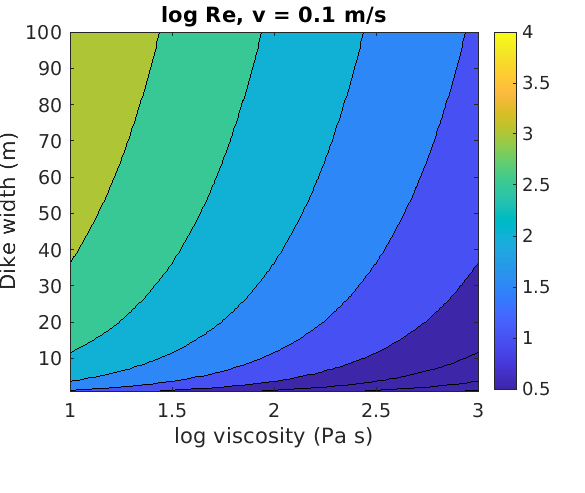
\includegraphics[scale=.5]{vpoint1.png}

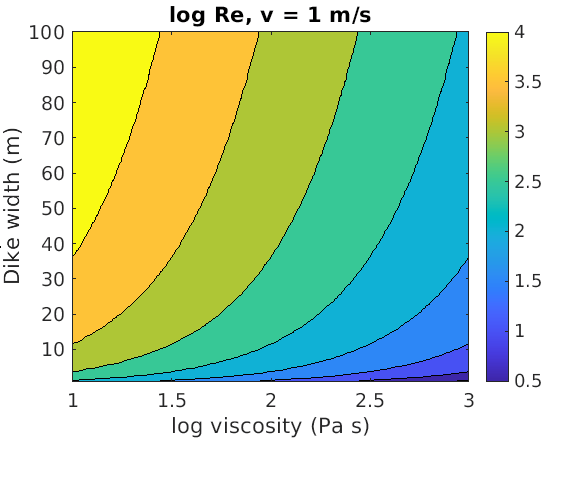
\includegraphics[scale=.5]{v1.png}

\newpage

\noindent\textbf{Problem 4}
\begin{enumerate}
\item\begin{gather*}
  \rho \frac{\partial v_1}{\partial t} = - \frac{\partial P}{\partial x_1} + \eta \left(\frac{\partial^2 v_1}{\partial x_1 ^ 2} + \frac{\partial^2 v_1}{\partial x_2 ^ 2} + \frac{\partial^2 v_1}{\partial x_3 ^ 2}\right) + \rho g_1\\
  \rho \frac{\partial v_2}{\partial t} = - \frac{\partial P}{\partial x_1} + \eta \left(\frac{\partial^2 v_2}{\partial x_1 ^ 2} + \frac{\partial^2 v_2}{\partial x_2 ^ 2} + \frac{\partial^2 v_2}{\partial x_3 ^ 2}\right) + \rho g_2\\
    \rho \frac{\partial v_3}{\partial t} = - \frac{\partial P}{\partial x_1} + \eta \left(\frac{\partial^2 v_3}{\partial x_1 ^ 2} + \frac{\partial^2 v_3}{\partial x_2 ^ 2} + \frac{\partial^2 v_3}{\partial x_3 ^ 2}\right) + \rho g_3\\
\end{gather*}
\item
  $\nabla P = \begin{bmatrix}
  \frac{\partial P}{\partial x_1}\\
  \frac{\partial P}{\partial x_2}\\
  \frac{\partial P}{\partial x_3}\\
  \end{bmatrix}$\\
\item$\nabla^2 v_{x_1} = \nabla\cdot\nabla v_{x_1} =\frac{\partial^2 v_{x_1}}{\partial x_1 ^2} +  \frac{\partial^2 v_{x_1}}{\partial x_2 ^2} +  \frac{\partial^2 v_{x_1}}{\partial x_3 ^2}$

\item $\rho \frac{\partial\vec{v}}{\partial t} = - \nabla P + \eta \nabla^2 \vec{v} + p\vec{g}$

  
\end{enumerate}

\end{document}
